
\section{自然标记拟范畴中的同构}\label{sec:isomorphisms-naturally-marked-quasi-categories}

由\cref{ex:maximally-marked-kan}，\trKanComplex{}可以视为复状单纯集的一个
特例：也就是说，\trKanComplex{}恰与那些极大标记的复状单纯集相重合。在本节中，
我们将发现\trQuasiCategory{}同样可以与某些 1-平凡的复状单纯集（见\cref{def:n-trivial}）
相认同，其中带标记的 1-\trSimplex{}由底\trSimplicialSet{}所确定。在\cref{thm:natural-marking-complicial}中，
我们证明\trQuasiCategory{}的\trCategory{}可以与那些带标记 1-\trSimplex{}在某种
即将引入的精确意义下\emph{饱和}的 1-平凡复状单纯集相认同。

复状单纯集中 1-\trSimplex{}上的诸标记不能随意指派：每一条带标记的边都必须是
我们现在引入的意义下的一个\trEquivalence。

\begin{definition}[\trEquivalence]\label{def:equivalence-marked-simplicial-set}
带标记\trSimplicialSet{}中的一个 1-\trSimplex{} $f$ 是一个\textbf{\trEquivalence}，
若存在如下图所示的一对薄 2-\trSimplex：
\begin{center}
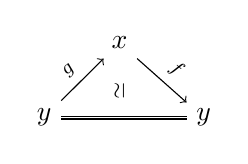
\begin{tikzpicture}[x=1.6em,y=1.35em]
  \node (x) at (1.7,2.0) {$x$};
  \node (yl) at (0,0) {$y$};
  \node (yr) at (3.6,0) {$y$};
  \draw[->] (yl) -- node[above,sloped,pos=0.45]{$\scriptstyle g$} (x);
  \draw[->] (x) -- node[above,sloped,pos=0.55]{$\scriptstyle f$} (yr);
  \draw[double] (yl) -- (yr);
  \node[rotate=90] at (1.7,0.72) {$\scriptstyle\simeq$};
\end{tikzpicture}
\qquad
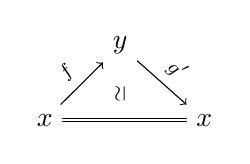
\begin{tikzpicture}[x=1.6em,y=1.35em]
  \node (y) at (1.7,2.0) {$y$};
  \node (xl) at (0,0) {$x$};
  \node (xr) at (3.6,0) {$x$};
  \draw[->] (xl) -- node[above,sloped,pos=0.45]{$\scriptstyle f$} (y);
  \draw[->] (y) -- node[above,sloped,pos=0.55]{$\scriptstyle g'$} (xr);
  \draw[double] (xl) -- (xr);
  \node[rotate=90] at (1.7,0.72) {$\scriptstyle\simeq$};
\end{tikzpicture}
\end{center}
\end{definition}

注意，\trEquivalence{}这一概念是相对于 2-\trSimplex{}上标记方式的选取而定义的。
对于\trQuasiCategory{}的边，一个非常相近的概念已在第 1 章中的\cref{def:isomorphism-quasi-category}
以「\trIsomorphism」之名得到定义。

\begin{lemma}\label{lem:marked-edges-equivalences}
复状单纯集中的每一条带标记的边都是一个\trEquivalence。
\end{lemma}

\begin{proof}
若 $f$ 是任一复状单纯集 $A$ 中的一条带标记的边，则第 0 面为 $f$ 而第 1 面
退化的那个 $\Lambda^{2}[2]$-\trHorn{}是容许的，故 $f$ 有一个右\trEquivalence{}逆。
一个涉及 $\Lambda^{0}[2]$-\trHorn{}的对偶构造表明 $f$ 还有一个左\trEquivalence{}逆：%
\footnote{又请注意，诸复状薄性扩张进一步蕴含这些单侧逆同样被标记，从而它们
容有各自的进一步的逆。}
\begin{center}
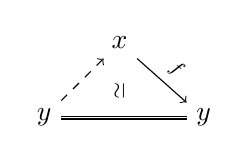
\begin{tikzpicture}[x=1.6em,y=1.35em]
  \node (x) at (1.7,2.0) {$x$};
  \node (yl) at (0,0) {$y$};
  \node (yr) at (3.6,0) {$y$};
  \draw[->,dashed] (yl) -- (x);
  \draw[->] (x) -- node[above,sloped,pos=0.55]{$\scriptstyle f$} (yr);
  \draw[double] (yl) -- (yr);
  \node[rotate=90] at (1.7,0.72) {$\scriptstyle\simeq$};
\end{tikzpicture}
\qquad
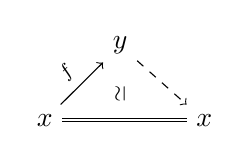
\begin{tikzpicture}[x=1.6em,y=1.35em]
  \node (y) at (1.7,2.0) {$y$};
  \node (xl) at (0,0) {$x$};
  \node (xr) at (3.6,0) {$x$};
  \draw[->] (xl) -- node[above,sloped,pos=0.45]{$\scriptstyle f$} (y);
  \draw[->,dashed] (y) -- (xr);
  \draw[double] (xl) -- (xr);
  \node[rotate=90] at (1.7,0.72) {$\scriptstyle\simeq$};
\end{tikzpicture}
\end{center}
\end{proof}

这一观察提示了给 1-\trCategory{}的\trNerve{}的边作标记的两种方式。

\begin{lemma}\label{lem:nerve-1-category-complicial}
一个 1-\trCategory{}的\trNerve{}定义一个复状单纯集，此时标记维数大于一的全部%
\trSimplex，然后以下列两种方式之一定义带标记的边：
\begin{enumerate}[label=(\roman*)]
\item 带标记的边仅为诸恒同箭头；或者
\item 带标记的边为全部\trIsomorphism。
\end{enumerate}
\end{lemma}

\begin{proof}
见\cref{ex:prove-lem-nerve-1-category}。
\end{proof}

这两种选取中的前者定义了使 1-\trCategory{}的\trNerve{}成为复状单纯集的极小
1-平凡标记。据\cref{lem:marked-edges-equivalences}，后者定义了使 1-\trCategory{}%
的\trNerve{}成为复状单纯集的极大标记。我们现在引入一套术语来描述「极大标记的」
1-平凡复状单纯集。

\begin{definition}[1-饱和的]\label{def:1-saturated}
一个复状单纯集是 \textbf{1-饱和的}（1-saturated），若它的诸边之中所含的每一个%
\trEquivalence{}都被标记。\footnote{由于在诸 1-\trSimplex{}之中刻画\trEquivalence{}%
需要预先约定哪些 2-\trSimplex{}被标记，我们通常将\cref{def:1-saturated}应用于
1-平凡的复状单纯集；此时我们简称一个 1-饱和的 1-平凡复状单纯集为「饱和的」
（saturated）。这是\cref{dig:saturation-higher-simplices}中所讨论的饱和复状
单纯集这一一般概念的一个特例。}
\end{definition}

这促成了下述\trQuasiCategory{}之典范标记的定义——它在 \cite{bib78} 中称作
「自然标记」。也就是说，我们赋予每个\trQuasiCategory{}其唯一的 1-饱和 1-平凡
标记：

\begin{definition}[自然标记]\label{def:natural-marking}
对任何\trQuasiCategory{} $A$，其\textbf{自然标记}定义如下：
\begin{itemize}
\item 标记维数大于一的全部\trSimplex{}；
\item 恰好标记那些作为\trIsomorphism{}的边（第 1 章中的\cref{def:isomorphism-quasi-category}
  的意义下），或者等价地，标记全部那些作为\trEquivalence{}的边
  （\cref{def:equivalence-marked-simplicial-set} 的意义下）。
\end{itemize}
\end{definition}

\trQuasiCategory{}的自然标记便于陈述并证明一个归功于 Joyal 的重要组合结果：

\begin{proposition}\label{prop:outer-complicial-horn-fillings}
任何自然标记\trQuasiCategory{} $A$ 对 $n\ge 1$ 容有外复状号角扩张的\trFiller：
\begin{center}
\begin{tikzpicture}[x=1.6em,y=1.4em]
  \node (lt) at (0,1.2) {$\Lambda^{0}[n]$};
  \node (rt) at (2.8,1.2) {$A$};
  \node (lb) at (0,-1.2) {$\Delta^{0}[n]$};
  \draw[->] (lt) -- (rt);
  \draw[right hook->] (lb) -- (lt);
  \node at (-0.45,0) {$\scriptstyle r$};
  \draw[->,dashed] (0.45,-1.0) -- (2.35,1.0);
\end{tikzpicture}
\qquad
\begin{tikzpicture}[x=1.6em,y=1.4em]
  \node (lt) at (0,1.2) {$\Lambda^{n}[n]$};
  \node (rt) at (2.8,1.2) {$A$};
  \node (lb) at (0,-1.2) {$\Delta^{n}[n]$};
  \draw[->] (lt) -- (rt);
  \draw[right hook->] (lb) -- (lt);
  \node at (-0.45,0) {$\scriptstyle r$};
  \draw[->,dashed] (0.45,-1.0) -- (2.35,1.0);
\end{tikzpicture}
\end{center}
\end{proposition}

在原始文献 \cite{bib61} 中，该结果不带标记地陈述如下：一个\trQuasiCategory{}%
对\textbf{特殊外\trHorn}容有\trFiller——即初始 $\{01\}$-边被映成 $A$ 中一个%
\trIsomorphism{}的左\trHorn{} $\Lambda^{0}[n]\to A$，以及末端 $\{n{-}1\,n\}$-边
被映成 $A$ 中一个\trIsomorphism{}的右\trHorn{} $\Lambda^{n}[n]\to A$。

\cref{prop:outer-complicial-horn-fillings}的诸多证明都是可能的；例如见
\cite[\S B]{bib36} 或原始文献 \cite{bib61}。我们选择采用 \trVerity{}的组合结果
\cite[\S4.2]{bib129}，并分期予以陈述；这些结果使用了\trHomotopyCoherentIsomorphism
的一个替代概念（事后可见与之等价）——同伦类型论家会凭「半伴随等价」
（half adjoint equivalence）之名认出它 \cite[\S4.2]{bib125}。

\begin{notation}[相干同构的子复形]\label{not:subcomplexes-coherent-isomorphism}
回顾\textbf{相干同构}（coherent isomorphism）：即定义为\trFreeLivingIsomorphism
之\trNerve{}的那个\trSimplicialSet{} $\qcInt$。它在每一维恰有两个非退化%
\trSimplex。若把它的顶点标作「$-$」与「$+$」，则其余非退化\trSimplex{}便由其
顶点唯一确定，这些顶点即从任一端出发的「$-$」与「$+$」的交错序列。作为%
\trMarkedSimplicialSet，我们赋予 $\qcInt$ 及其子复形（subcomplexes）极大标记。
\end{notation}

沿 \cite{bib129,bib42} 引入的记号，我们记 $E_{n}^{\pm}$、$E_{n}^{\mp}\subset\qcInt$
为分别由 $n$-\trSimplex{} $-+-\cdots\pm$ 与 $+-+\cdots\mp$ 生成的单纯子集。两个
单纯子集均唯一地嵌入 $E_{n+1}^{\mp}$ 与 $E_{n+1}^{\pm}$ 两者，且这些包含按如下
方式分解
\begin{center}
\begin{tikzpicture}[x=1.05em,y=1.3em]
  \node (lt1) at (0,3.2) {$\Lambda^{0}[n+1]$};
  \node (rt1) at (5.4,3.2) {$E_{n}^{\pm}$};
  \node (lb1) at (0,1.0) {$\Delta^{0}[n+1]$};
  \node (bul1) at (5.4,1.0) {$\bullet$};
  \node (rb1) at (10.8,1.0) {$\Delta^{0}[n+1]'$};
  \node (bb1) at (5.4,-1.4) {$E_{n+1}^{\pm}$};
  \node (rb2) at (10.8,-1.4) {$\Delta^{0}[n+1]''$};
  \draw[->] (lt1) -- (rt1);
  \draw[right hook->] (lb1) -- node[pos=0.5,left]{$\scriptstyle r$} (lt1);
  \draw[right hook->] (rt1) -- (bul1);
  \draw[->] (lb1) -- (bul1);
  \node at (4.75,1.28) {$\scriptstyle\llcorner$};
  \draw[->] (rb1) -- (bul1);
  \draw[->] (bul1) -- (bb1);
  \node at (4.75,-0.95) {$\scriptstyle\llcorner$};
  \draw[right hook->] (rb2) -- node[pos=0.5,right]{$\scriptstyle e$} (rb1);
  \draw[->] (rb2) -- (bb1);
  \node (lt2) at (14.0,3.2) {$\Lambda^{n+1}[n+1]$};
  \node (rt2) at (20.6,3.2) {$E_{n}^{\pm}$};
  \node (lb2) at (14.0,1.0) {$\Delta^{n+1}[n+1]$};
  \node (bul2) at (20.6,1.0) {$\bullet$};
  \node (rb3) at (27.2,1.0) {$\Delta^{n+1}[n+1]'$};
  \node (bb2) at (20.6,-1.4) {$E_{n+1}^{\pm}$};
  \node (rb4) at (27.2,-1.4) {$\Delta^{n+1}[n+1]''$};
  \draw[->] (lt2) -- (rt2);
  \draw[right hook->] (lb2) -- node[pos=0.5,left]{$\scriptstyle r$} (lt2);
  \draw[right hook->] (rt2) -- (bul2);
  \draw[->] (lb2) -- (bul2);
  \node at (19.95,1.28) {$\scriptstyle\llcorner$};
  \draw[->] (rb3) -- (bul2);
  \draw[->] (bul2) -- (bb2);
  \node at (19.95,-0.95) {$\scriptstyle\llcorner$};
  \draw[right hook->] (rb4) -- node[pos=0.5,right]{$\scriptstyle e$} (rb3);
  \draw[->] (rb4) -- (bb2);
\end{tikzpicture}
\end{center}
从而证明了任何满足 $m>n$ 的包含 $E_{n}^{\pm}\hookrightarrow E_{m}^{\pm}$ 或
$E_{n}^{\mp}\hookrightarrow E_{m}^{\pm}$ 都是带标记\trAnodyneExtension。

下述结果给出一个判据，用以断定一个\textbf{内复状纤维化}（inner complicial
fibration）——即只假定了对诸内复状号角扩张与诸内复状薄性扩张具有右提升性质的
带标记映射——何时在事实上定义一个复状等价纤维化。

\begin{proposition}\label{prop:inner-complicial-fibration-criterion}
设 $p\colon A\twoheadrightarrow B$ 是一个内复状纤维化，其余定义域 $B$ 是一个
复状单纯集。则 $p$ 是一个复状等价纤维化，当且仅当 $p$ 对包含
$E_{0}^{-}\hookrightarrow E_{1}^{-}$ 与 $E_{1}^{-}\hookrightarrow E_{3}^{-}$
容有提升。
\end{proposition}

\begin{proof}
任何复状等价纤维化都对带标记\trAnodyneExtension $E_{0}^{-}\hookrightarrow E_{1}^{-}$ 与
$E_{1}^{-}\hookrightarrow E_{3}^{-}$ 容有提升。于是，本结果的核心，也是唯一
尚待证明的部分，即是如下断言：任何对这一对包含容有提升、且余定义域为复状
单纯集的内复状纤维化，必然也对外复状号角扩张与外复状薄性扩张容有\trFiller。

我们先论证：满足陈述条件的内复状纤维化 $p\colon A\twoheadrightarrow B$ 也对
对偶包含 $E_{0}^{-}\hookrightarrow E_{1}^{+}$ 容有提升。给定如下方块中由映射
$a$ 与 $b$ 呈现的提升问题：
\begin{center}
\begin{tikzpicture}[x=1.6em,y=1.4em]
  \node (e0) at (0.6,2.4) {$E_{0}^{-}$};
  \node (A)  at (4.4,2.4) {$A$};
  \node (e1m) at (-2.4,0.7) {$E_{1}^{-}$};
  \node (e1p) at (0.6,0.7) {$E_{1}^{+}$};
  \node (B)  at (4.4,0.7) {$B$};
  \node (e3) at (0.6,-1.5) {$E_{3}^{-}$};
  \draw[->] (e1m) -- (e0);
  \draw[->] (e1m) -- (e3);
  \draw[right hook->] (e0) -- (e1p);
  \draw[right hook->] (e1p) -- (e3);
  \draw[->] (e0) -- node[above]{$\scriptstyle a$} (A);
  \draw[->] (e1p) -- node[above]{$\scriptstyle b$} (B);
  \draw[->] (A) -- node[right]{$\scriptstyle p$} (B);
  \draw[->,dashed] (e3) -- (B);
  \draw[->,dotted] (e1p) -- (A);
\end{tikzpicture}
\end{center}
则存在 $b$ 沿 $E_{1}^{+}\hookrightarrow E_{3}^{-}$ 的虚线\trExtension，因为该
包含是带标记\trAnodyneExtension{}且 $B$ 是复状单纯集。现在，包含 $E_{0}^{-}\hookrightarrow E_{3}^{-}$
如所示分解为 $E_{0}^{-}\hookrightarrow E_{1}^{+}\hookrightarrow E_{3}^{-}$，而
由假设 $p$ 对这两个映射均可提升，故点线提升也存在，它经限制便定义了原提升问题
的一个解。

手持这一结果，立即可知 $p\colon A\twoheadrightarrow B$ 的奇对偶满足与
$p\colon A\twoheadrightarrow B$ 相同的提升性质，因为 $E_{0}^{-}\hookrightarrow E_{1}^{-}$
的奇对偶是 $E_{0}^{-}\hookrightarrow E_{1}^{+}$，而 $E_{1}^{-}\hookrightarrow E_{3}^{-}$
的奇对偶同构于其自身。于是只须证明：$p$ 对左复状号角扩张
$\Lambda^{0}[n]\hookrightarrow_{r}\Delta^{0}[n]$ 与左复状薄性扩张
$\Delta^{0}[n]'\hookrightarrow_{e}\Delta^{0}[n]''$ 容有提升即可，此时其奇对偶
将分享这些性质，这蕴含 $p$ 对右复状号角扩张与右复状薄性扩张也容有提升。情形
$\Lambda^{0}[1]\hookrightarrow\Delta^{0}[1]$ 即映射 $E_{0}^{-}\hookrightarrow E_{1}^{-}$，
故还可设 $n>1$，此时我们有同构
\[
\Lambda^{0}[n]\hookrightarrow\Delta^{0}[n]
\cong(\Lambda^{0}[1]\hookrightarrow\Delta^{0}[1])\mathbin{\hat{\star}}
(\partial\Delta[n-2]\hookrightarrow\Delta[n-2])\text{，}
\]
由\cref{lem:leibniz-join-complicial}。为简便计记 $m=n-2$，考虑由映射 $a$ 与
$b$ 呈现的提升问题：
\begin{center}
\begin{tikzpicture}[x=1.0em,y=1.4em]
  \node (tl) at (0,1.7) {$E_{0}^{-}\star\Delta[m]\cup E_{1}^{-}\star\partial\Delta[m]$};
  \node (tr) at (14.6,1.7) {$A$};
  \node (bl) at (0,-0.7) {$E_{1}^{-}\star\Delta[m]$};
  \node (bm) at (7.3,-0.7) {$E_{2}^{-}\star\Delta[m]_{t}\cup E_{3}^{-}\star\partial\Delta[m]$};
  \node (br) at (14.6,-0.7) {$E_{3}^{-}\star\Delta[m]$};
  \node (B) at (17.2,-0.7) {$B$};
  \draw[->] (tl) -- node[above]{$\scriptstyle a$} (tr);
  \draw[right hook->] (tl) -- node[pos=0.45,left]{$\scriptstyle i$} (bl);
  \draw[right hook->] (bl) -- (bm);
  \draw[right hook->] (bm) -- (br);
  \draw[->,dashed] (br) -- (B);
  \draw[->] (tr) -- node[right]{$\scriptstyle p$} (B);
  \draw[->,dotted] (bm) -- (tr);
  \draw[->] (bl) to[bend right=12] node[below,pos=0.55]{$\scriptstyle j$} (br);
  \draw[->] (bl) to[bend right=20] node[below,pos=0.55]{$\scriptstyle b$} (B);
\end{tikzpicture}
\end{center}
据\cref{lem:leibniz-join-complicial}，映射 $j$ 是带标记\trAnodyneExtension，故由于 $B$ 是
复状单纯集，虚线\trExtension{}存在。为证明点线提升也存在，我们论证：映射 $i$
由诸内复状号角扩张与映射 $E_{1}^{-}\hookrightarrow E_{3}^{-}$ 胞腔式生成。为
看到这一点，将映射 $i$ 分解为

\begin{rveq}\label{eq:pushout-squares-factorization}
\begin{tikzpicture}[x=1.0em,y=1.35em]
  \node (a) at (0,3.4) {$E_{1}^{-}$};
  \node (b) at (7.0,3.4) {$E_{0}^{-}\star\Delta[m]\cup E_{1}^{-}\star\partial\Delta[m]$};
  \node (c) at (0,1.7) {$E_{3}^{-}$};
  \node (d) at (7.0,1.7) {$\bullet$};
  \node (e) at (14.6,1.7) {$E_{1}^{-}\star\partial\Delta[m]\cup E_{3}^{-}\star\varnothing$};
  \node (f) at (0,0) {$E_{0}^{-}\star\Delta[m]\cup E_{2}^{-}\star\partial\Delta[m]$};
  \node (g) at (7.0,0) {$\bullet$};
  \node (h) at (14.6,0) {$E_{3}^{-}\star\partial\Delta[m]$};
  \node (i) at (0,-1.7) {$E_{2}^{-}\star\Delta[m]$};
  \node (j) at (7.0,-1.7) {$E_{2}^{-}\star\Delta[m]\cup E_{3}^{-}\star\partial\Delta[m]$};
  \draw[right hook->] (a) -- (b);
  \draw[right hook->] (a) -- (c);
  \draw[right hook->] (b) -- (d);
  \draw[->] (c) -- (d);
  \node at (6.35,1.95) {$\scriptstyle\llcorner$};
  \draw[right hook->] (e) -- (d);
  \draw[->] (d) -- (g);
  \draw[right hook->] (e) -- (h);
  \draw[->] (h) -- (g);
  \node at (6.35,0.25) {$\scriptstyle\llcorner$};
  \draw[right hook->] (f) -- (g);
  \draw[right hook->] (f) -- (i);
  \draw[->] (g) -- (j);
  \draw[right hook->] (i) -- (j);
  \node at (6.35,-1.4) {$\scriptstyle\llcorner$};
\end{tikzpicture}
\end{rveq}

第一个附贴胞腔就是映射 $E_{1}^{-}\hookrightarrow E_{3}^{-}$ 本身。如
\cref{not:subcomplexes-coherent-isomorphism} 中所观察，$E_{1}^{-}\hookrightarrow E_{3}^{-}$
是一个右\trAnodyneExtension，故据\cref{lem:leibniz-join-complicial}，第二个附贴胞腔
$(E_{1}^{-}\hookrightarrow E_{3}^{-})\mathbin{\hat{\star}}(\varnothing\hookrightarrow\partial\Delta[m])$
是一个内\trAnodyneExtension。类似地 $E_{0}^{-}\hookrightarrow E_{2}^{-}$ 是一个右\trAnodyneExtension，
故最后一个附贴胞腔
$(E_{0}^{-}\hookrightarrow E_{2}^{-})\mathbin{\hat{\star}}(\partial\Delta[m]\hookrightarrow\Delta[m])$
也是一个内\trAnodyneExtension。从而，$p$ 对诸左复状号角扩张容有提升，如所断言。

为看出 $p\colon A\to B$ 也对外复状薄性扩张容有提升，我们利用\cref{lem:leibniz-join-complicial}
的下述同构
\[
(\Lambda^{0}[1]\hookrightarrow\Delta^{0}[1])\mathbin{\hat{\star}}(\Delta[m]\hookrightarrow\Delta[m]_{t})
\cong
\Delta^{0}[m+2]'\hookrightarrow\Delta^{0}[m+2]''\text{，}
\]
忆及 $\Lambda^{0}[1]\hookrightarrow\Delta^{0}[1]$ 即包含 $E_{0}^{-}\hookrightarrow E_{1}^{-}$。
于是我们可以考虑由映射 $a$ 与 $b$ 呈现的提升问题：
\begin{center}
\begin{tikzpicture}[x=1.0em,y=1.4em]
  \node (tl) at (0,1.7) {$E_{0}^{-}\star\Delta[m]_{t}\cup E_{1}^{-}\star\Delta[m]$};
  \node (tr) at (14.6,1.7) {$A$};
  \node (bl) at (0,-0.7) {$E_{1}^{-}\star\Delta[m]_{t}$};
  \node (bm) at (7.3,-0.7) {$E_{2}^{-}\star\Delta[m]\cup E_{3}^{-}\star\Delta[m]$};
  \node (br) at (14.6,-0.7) {$E_{3}^{-}\star\Delta[m]_{t}$};
  \node (B) at (17.2,-0.7) {$B$};
  \draw[->] (tl) -- node[above]{$\scriptstyle a$} (tr);
  \draw[right hook->] (tl) -- node[pos=0.45,left]{$\scriptstyle i$} (bl);
  \draw[right hook->] (bl) -- (bm);
  \draw[right hook->] (bm) -- (br);
  \draw[->,dashed] (br) -- (B);
  \draw[->] (tr) -- node[right]{$\scriptstyle p$} (B);
  \draw[->,dotted] (bm) -- (tr);
  \draw[->] (bl) to[bend right=12] node[below,pos=0.55]{$\scriptstyle j$} (br);
  \draw[->] (bl) to[bend right=20] node[below,pos=0.55]{$\scriptstyle b$} (B);
\end{tikzpicture}
\end{center}
据\cref{lem:leibniz-join-complicial}，映射 $j$ 是带标记\trAnodyneExtension，故由于 $B$ 是
复状单纯集，虚线\trExtension{}存在。为证明点线提升也存在，我们论证：映射 $i$
由诸内复状号角扩张、诸内复状薄性扩张与映射 $E_{1}^{-}\hookrightarrow E_{3}^{-}$
胞腔式生成。为看到这一点，将映射 $i$ 分解为

\begin{center}
\begin{tikzpicture}[x=1.0em,y=1.35em]
  \node (a) at (0,3.4) {$E_{1}^{-}$};
  \node (b) at (7.0,3.4) {$E_{0}^{-}\star\Delta[m]_{t}\cup E_{1}^{-}\star\Delta[m]$};
  \node (c) at (0,1.7) {$E_{3}^{-}$};
  \node (d) at (7.0,1.7) {$\bullet$};
  \node (e) at (14.6,1.7) {$E_{1}^{-}\star\Delta[m]\cup E_{3}^{-}\star\varnothing$};
  \node (f) at (0,0) {$E_{0}^{-}\star\Delta[m]_{t}\cup E_{2}^{-}\star\Delta[m]$};
  \node (g) at (7.0,0) {$\bullet$};
  \node (h) at (14.6,0) {$E_{3}^{-}\star\Delta[m]$};
  \node (i) at (0,-1.7) {$E_{2}^{-}\star\Delta[m]_{t}$};
  \node (j) at (7.0,-1.7) {$E_{2}^{-}\star\Delta[m]_{t}\cup E_{3}^{-}\star\Delta[m]$};
  \draw[right hook->] (a) -- (b);
  \draw[right hook->] (a) -- (c);
  \draw[right hook->] (b) -- (d);
  \draw[->] (c) -- (d);
  \node at (6.35,1.95) {$\scriptstyle\llcorner$};
  \draw[right hook->] (e) -- (d);
  \draw[->] (d) -- (g);
  \draw[right hook->] (e) -- (h);
  \draw[->] (h) -- (g);
  \node at (6.35,0.25) {$\scriptstyle\llcorner$};
  \draw[right hook->] (f) -- (g);
  \draw[right hook->] (f) -- (i);
  \draw[->] (g) -- (j);
  \draw[right hook->] (i) -- (j);
  \node at (6.35,-1.4) {$\scriptstyle\llcorner$};
\end{tikzpicture}
\end{center}

第一个附贴胞腔就是映射 $E_{1}^{-}\hookrightarrow E_{3}^{-}$ 本身。如
\cref{not:subcomplexes-coherent-isomorphism} 中所观察，$E_{1}^{-}\hookrightarrow E_{3}^{-}$
是一个右带标记\trAnodyneExtension，故据\cref{lem:leibniz-join-complicial}，第二个附贴胞腔
$(E_{1}^{-}\hookrightarrow E_{3}^{-})\mathbin{\hat{\star}}(\varnothing\hookrightarrow\Delta[m])$
是一个内带标记\trAnodyneExtension。类似地 $E_{0}^{-}\hookrightarrow E_{2}^{-}$ 是一个右%
\trAnodyneExtension，故最后一个附贴胞腔
$(E_{0}^{-}\hookrightarrow E_{2}^{-})\mathbin{\hat{\star}}(\Delta[m]\hookrightarrow\Delta[m]_{t})$
也是一个内复状薄性扩张。从而，$p$ 对诸左复状薄性扩张容有提升，如所断言。
\end{proof}

由于包含 $E_{0}^{-}\hookrightarrow E_{1}^{-}$ 与 $E_{1}^{-}\hookrightarrow E_{3}^{-}$
是左带标记\trAnodyneExtension，\cref{prop:inner-complicial-fibration-criterion} 立得下述
推论。

\begin{corollary}\label{cor:left-right-complicial-fibration}
设 $p\colon A\twoheadrightarrow B$ 是一个内复状纤维化，其余定义域 $B$ 是一个
复状单纯集。则当 $p$ 是一个左复状纤维化或一个右复状纤维化时，$p$ 是一个复状
等价纤维化。
\end{corollary}

请注意，在\cref{prop:inner-complicial-fibration-criterion}的证明中，对包含
$E_{0}^{-}\hookrightarrow E_{1}^{-}$ 的提升只是在构造外复状号角扩张
$\Lambda^{0}[1]\hookrightarrow\Delta^{0}[1]$ 与 $\Lambda^{1}[1]\hookrightarrow\Delta^{1}[1]$
的提升时才需要。于是，即便去掉这一提升条件，更高维数的外复状号角扩张仍可
构造出来。刚才给出的论证给出了「特殊外\trHorn{}填充」的一个特例的证明，这一
特例在证明一般版本时有用。

\begin{lemma}\label{lem:left-horn-filling-degenerate-edge}
设 $p\colon A\twoheadrightarrow B$ 是一个内复状纤维化，其余定义域 $B$ 是一个
复状单纯集。则 $p$ 对左\trHorn
\begin{center}
\begin{tikzpicture}[x=1.6em,y=1.4em]
  \node (lt) at (0,1.2) {$\Lambda^{0}[n]$};
  \node (rt) at (2.8,1.2) {$A$};
  \node (lb) at (0,-1.2) {$\Delta^{0}[n]$};
  \node (rb) at (2.8,-1.2) {$B$};
  \draw[->] (lt) -- node[above]{$\scriptstyle a$} (rt);
  \draw[right hook->] (lb) -- (lt);
  \draw[->] (lb) -- node[below]{$\scriptstyle b$} (rb);
  \draw[->] (rt) -- node[right]{$\scriptstyle p$} (rb);
  \draw[->,dashed] (0.45,-1.0) -- (2.35,1.0);
\end{tikzpicture}
\end{center}
（$n>1$）容有\trFiller，只要 $a$ 把\trHorn{} $\Lambda^{0}[n]$ 的 $\{01\}$ 边
送到 $A$ 中一个退化\trSimplex。
\end{lemma}

\begin{proof}
记 $m=n-2$。据\cref{lem:leibniz-join-complicial}，我们有同构
\[
\Lambda^{0}[m+2]\hookrightarrow\Delta^{0}[m+2]
\cong(\Lambda^{0}[1]\hookrightarrow\Delta^{0}[1])\mathbin{\hat{\star}}
(\partial\Delta[m]\hookrightarrow\Delta[m])\text{，}
\]
于是我们再一次被要求考虑由映射 $a$ 与 $b$ 呈现的提升问题：
\begin{center}
\begin{tikzpicture}[x=1.0em,y=1.4em]
  \node (tl) at (0,1.9) {$E_{0}^{-}\star\Delta[m]\cup E_{1}^{-}\star\partial\Delta[m]$};
  \node (tm) at (8.2,1.9) {$E_{0}^{-}\star\Delta[m]\cup E_{1}^{-}\star\partial\Delta[m]\underset{E_{1}^{-}}{\cup}E_{3}^{-}$};
  \node (tr) at (17.4,1.9) {$A$};
  \node (bl) at (0,-0.9) {$E_{1}^{-}\star\Delta[m]$};
  \node (bm) at (8.2,-0.9) {$E_{2}^{-}\star\Delta[m]\cup E_{3}^{-}\star\partial\Delta[m]$};
  \node (br) at (17.4,-0.9) {$E_{3}^{-}\star\Delta[m]$};
  \node (B) at (20.0,-0.9) {$B$};
  \draw[->] (tl) to[bend left=18] node[above,pos=0.4]{$\scriptstyle a$} (tr);
  \draw[right hook->] (tl) -- node[below,pos=0.5]{$\scriptstyle k$} (tm);
  \draw[->,dashed] (tm) -- (tr);
  \draw[right hook->] (tl) -- node[pos=0.45,left]{$\scriptstyle i$} (bl);
  \draw[right hook->] (tm) -- node[pos=0.45,right]{$\scriptstyle\ell$} (bm);
  \draw[right hook->] (bl) -- (bm);
  \draw[right hook->] (bm) -- (br);
  \draw[->,dashed] (br) -- (B);
  \draw[->] (tr) -- node[right]{$\scriptstyle p$} (B);
  \draw[->,dotted] (bm) -- (tr);
  \draw[->] (bl) to[bend right=12] node[below,pos=0.55]{$\scriptstyle j$} (br);
  \draw[->] (bl) to[bend right=20] node[below,pos=0.55]{$\scriptstyle b$} (B);
\end{tikzpicture}
\end{center}
映射 $j$ 是带标记\trAnodyneExtension，故由于 $B$ 是复状单纯集，下方的虚线\trExtension{}%
存在，于是只剩下求解映射 $i$ 与映射 $p$ 之间的提升问题。为此，我们把映射 $i$
分解为 \eqref{eq:pushout-squares-factorization} 中所示的中间一列三个竖直态射的
复合，并令 $k$ 记这些态射中的第一个，而 $\ell$ 记后两个的复合。接下来，通过
指定被附贴的 $E_{3}^{-}$ 的像为一个退化 3-\trSimplex{}来求解 $k$ 与 $p$ 之间
的提升问题；注意 $k$ 的构造方式是把该 $E_{3}^{-}$ 附贴到对应于号角
$\Lambda^{0}[m+2]$ 之初始边的那只 $E_{1}^{-}$ 上，而 $a$ 把这条边送到一条退化边。

现在，为构造点线提升，只剩下求解 $\ell$ 与 $p$ 之间的提升问题，而
\eqref{eq:pushout-squares-factorization} 揭示这可以做到：它把映射 $\ell$ 表为
诸内复状号角扩张的推出之复合。
\end{proof}

\begin{corollary}\label{cor:inner-fillings-complicial-set}
一个对诸内复状号角扩张与诸内复状薄性扩张容有\trFiller{}的带标记\trSimplicialSet
$A$ 是一个复状单纯集，当且仅当它沿 $\Delta[1]^{\sharp}\hookrightarrow\mathrm{sk}_{2}\qcInt^{\sharp}$
容有\trExtension。
\end{corollary}

\begin{proof}
把\cref{prop:inner-complicial-fibration-criterion}应用于内复状纤维化
$A\to\qcOne$：为断定 $A$ 是一个复状单纯集，只须沿映射 $E_{0}^{-}\hookrightarrow E_{1}^{-}$
与 $E_{1}^{-}\hookrightarrow E_{3}^{-}$ 构造\trExtension。前者是自动的，因为
$E_{0}^{-}\hookrightarrow E_{1}^{-}$ 同构于 $\Delta[0]\hookrightarrow\Delta[1]^{\sharp}$，
而后者容有一个收缩，所以为完成证明，我们将表明：在所述假设下，若 $A$ 沿映射
$E_{1}^{-}\hookrightarrow E_{3}^{-}$ 容有\trExtension，则结论成立。

定义域映射 $\Delta[1]^{\sharp}\cong E_{1}^{-}\to A$ 定义 $A$ 中一个带标记
1-\trSimplex{} $f\colon x\to y$，据假设我们可以把它\trExtension{}成映射
$\mathrm{sk}_{2}\qcInt^{\sharp}\to A$，后者指明诸带标记 2-\trSimplex
\begin{center}
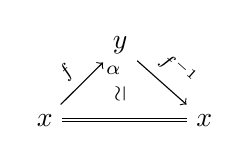
\begin{tikzpicture}[x=1.6em,y=1.35em]
  \node (y) at (1.7,2.0) {$y$};
  \node (xl) at (0,0) {$x$};
  \node (xr) at (3.6,0) {$x$};
  \draw[->] (xl) -- node[above,sloped,pos=0.45]{$\scriptstyle f$} (y);
  \draw[->] (y) -- node[above,sloped,pos=0.55]{$\scriptstyle f^{-1}$} (xr);
  \draw[double] (xl) -- (xr);
  \node at (1.55,1.35) {$\scriptstyle\alpha$};
  \node[rotate=90] at (1.7,0.72) {$\scriptstyle\simeq$};
\end{tikzpicture}
\qquad
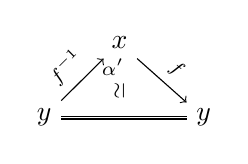
\begin{tikzpicture}[x=1.6em,y=1.35em]
  \node (x) at (1.7,2.0) {$x$};
  \node (yl) at (0,0) {$y$};
  \node (yr) at (3.6,0) {$y$};
  \draw[->] (yl) -- node[above,sloped,pos=0.45]{$\scriptstyle f^{-1}$} (x);
  \draw[->] (x) -- node[above,sloped,pos=0.55]{$\scriptstyle f$} (yr);
  \draw[double] (yl) -- (yr);
  \node at (1.55,1.35) {$\scriptstyle\alpha'$};
  \node[rotate=90] at (1.7,0.72) {$\scriptstyle\simeq$};
\end{tikzpicture}
\end{center}
2-\trSimplex{} $\alpha$ 与 $\alpha'$ 可以理解为定义二维\trEquivalence{}
$\alpha\colon\mathrm{id}_{x}\simeq f^{-1}f$ 与
$\alpha'\colon\mathrm{id}_{y}\simeq ff^{-1}$。$\alpha$ 与 $\alpha'$ 这一对
2-\trSimplex{}未必构成映射 $E_{3}^{-}\to A$ 的两个非退化 2-\trSimplex{}面——
那将等同于附加要求：三角恒等复合 $(\alpha')^{-1}f\cdot f\alpha$ \trEquivalence{}%
于 $\mathrm{id}_{f}$，\footnote{这正是为什么带标记\trSimplicialSet{} $E_{3}^{-}$
与 $E_{3}^{+}$ 或许可被称作「半伴随等价」的缘由。}但我们将构造 $\alpha'$ 的一个
替代 $\beta$，使得 $\alpha$ 与 $\beta$ 构成 $E_{3}^{-}\to A$ 的非退化
2-\trSimplex。\footnote{这应当与第 2 章中经由\cref{lem:minimal-adjunction-data}
的\cref{prop:adjoint-equivalences}之证明相对照。}

3-\trSimplex{} $E_{3}^{-}$ 将被构造为我们即将搭建的号角 $\Lambda^{2}[4]\to A$
之\trFiller{}的第 2 面。作为对下述构造的定向指引，我们先总结最终结果：
\begin{itemize}
\item 第 0、第 2 与第 3 个顶点将是 $x$，而第 1 与第 4 个顶点将是 $y$；
\item 全部边都将是 $\mathrm{id}_{x}$、$\mathrm{id}_{y}$、$f$ 或 $f^{-1}$，
  其位置由诸顶点唯一确定；
\item 面 $\{0,1,2\}$ 与 $\{0,1,3\}$ 是 $\alpha$，而面 $\{1,2,4\}$ 是 $\alpha'$；
\item 面 $\{0,2,3\}$、$\{0,1,4\}$、$\{0,3,4\}$ 与 $\{1,2,3\}$ 是退化的；而
\item 缺失的面 $\{0,2,4\}$（称作 $\gamma$）、$\{2,3,4\}$（称作 $\bar{\gamma}$）
  与 $\{1,3,4\}$（称作 $\beta$）将按此顺序填入，所需的 3-\trSimplex{} $E_{3}^{-}$
  即作为号角的第 2 面出现。
\end{itemize}

第 4 面是经退化而得的 3-\trSimplex{} $\alpha\sigma^{2}$。第 3 面通过填充如下图
所示的号角 $\Lambda^{1}[3]\to A$ 而构造：
\begin{center}
\mbox{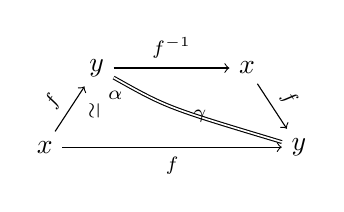
\begin{tikzpicture}[x=1.7em,y=1.3em]
  \node (yt) at (1.1,2.2) {$y$};
  \node (xt) at (4.3,2.2) {$x$};
  \node (xb) at (0,0) {$x$};
  \node (yb) at (5.4,0) {$y$};
  \draw[->] (xb) -- node[above,sloped,pos=0.45]{$\scriptstyle f$} (yt);
  \draw[->] (yt) -- node[above]{$\scriptstyle f^{-1}$} (xt);
  \draw[->] (xt) -- node[above,sloped,pos=0.55]{$\scriptstyle f$} (yb);
  \draw[->] (xb) -- node[below]{$\scriptstyle f$} (yb);
  \node at (1.5,1.45) {$\scriptstyle\alpha$};
  \node[rotate=90] at (1.05,1.0) {$\scriptstyle\simeq$};
  \draw[double] (yt) .. controls (2.6,1.1) .. (yb);
  \node at (3.3,0.85) {$\scriptstyle\gamma$};
\end{tikzpicture}}
\quad$\simeq$\quad
\mbox{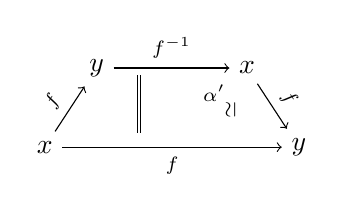
\begin{tikzpicture}[x=1.7em,y=1.3em]
  \node (yt) at (1.1,2.2) {$y$};
  \node (xt) at (4.3,2.2) {$x$};
  \node (xb) at (0,0) {$x$};
  \node (yb) at (5.4,0) {$y$};
  \draw[->] (xb) -- node[above,sloped,pos=0.45]{$\scriptstyle f$} (yt);
  \draw[->] (yt) -- node[above]{$\scriptstyle f^{-1}$} (xt);
  \draw[->] (xt) -- node[above,sloped,pos=0.55]{$\scriptstyle f$} (yb);
  \draw[->] (xb) -- node[below]{$\scriptstyle f$} (yb);
  \node at (3.6,1.5) {$\scriptstyle\alpha'$};
  \node[rotate=90] at (3.95,1.05) {$\scriptstyle\simeq$};
  \draw[double] (2.0,2.0) -- (2.0,0.4);
\end{tikzpicture}}
\end{center}
据一次复状薄性扩张，由填充该号角所定义的面 $\gamma$ 被标记。接着，第 1 面通过
填充号角 $\Lambda^{0}[3]\to A$ 构造，如\cref{lem:left-horn-filling-degenerate-edge}
所容许：

\begin{center}
\mbox{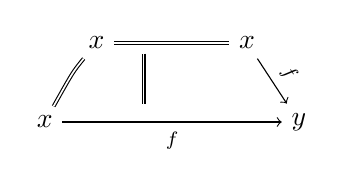
\begin{tikzpicture}[x=1.7em,y=1.3em]
  \node (xl) at (1.1,2.2) {$x$};
  \node (xr) at (4.3,2.2) {$x$};
  \node (xb) at (0,0) {$x$};
  \node (yb) at (5.4,0) {$y$};
  \draw[double] (xl) -- (xr);
  \draw[double] (xb) .. controls (0.6,1.4) .. (xl);
  \draw[->] (xr) -- node[above,sloped,pos=0.55]{$\scriptstyle f$} (yb);
  \draw[->] (xb) -- node[below]{$\scriptstyle f$} (yb);
  \draw[double] (2.1,1.9) -- (2.1,0.5);
  \node at (2.6,1.1) {$\scriptstyle\lVert$};
\end{tikzpicture}}
\quad$\simeq$\quad
\mbox{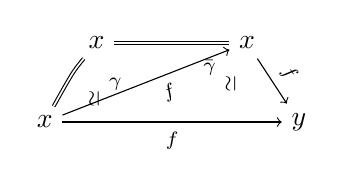
\begin{tikzpicture}[x=1.7em,y=1.3em]
  \node (xl) at (1.1,2.2) {$x$};
  \node (xr) at (4.3,2.2) {$x$};
  \node (xb) at (0,0) {$x$};
  \node (yb) at (5.4,0) {$y$};
  \draw[double] (xl) -- (xr);
  \draw[double] (xb) .. controls (0.6,1.4) .. (xl);
  \draw[->] (xr) -- node[above,sloped,pos=0.55]{$\scriptstyle f$} (yb);
  \draw[->] (xb) -- node[below]{$\scriptstyle f$} (yb);
  \draw[->] (xb) -- node[below,sloped,pos=0.6]{$\scriptstyle f$} (xr);
  \node at (1.5,1.05) {$\scriptstyle\gamma$};
  \node[rotate=90] at (1.05,0.65) {$\scriptstyle\simeq$};
  \node at (3.5,1.5) {$\scriptstyle\bar{\gamma}$};
  \node[rotate=90] at (3.95,1.05) {$\scriptstyle\simeq$};
\end{tikzpicture}}
\end{center}
这产生了另一个带标记 3-\trSimplex{} $\bar{\gamma}$，由填充该号角所定义。第 0 面
通过填充号角 $\Lambda^{1}[3]\to A$ 构造，如下图所示：
\begin{center}
\mbox{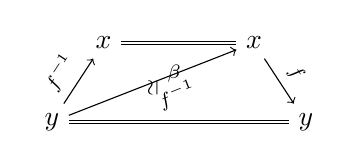
\begin{tikzpicture}[x=1.7em,y=1.3em]
  \node (xl) at (1.1,2.2) {$x$};
  \node (xr) at (4.3,2.2) {$x$};
  \node (yb) at (0,0) {$y$};
  \node (yr) at (5.4,0) {$y$};
  \draw[double] (xl) -- (xr);
  \draw[->] (yb) -- node[above,sloped,pos=0.45]{$\scriptstyle f^{-1}$} (xl);
  \draw[->] (xr) -- node[above,sloped,pos=0.55]{$\scriptstyle f$} (yr);
  \draw[double] (yb) -- (yr);
  \draw[->] (yb) -- node[below,sloped,pos=0.6]{$\scriptstyle f^{-1}$} (xr);
  \node at (2.6,1.35) {$\scriptstyle\beta$};
  \node[rotate=90] at (2.15,0.95) {$\scriptstyle\simeq$};
\end{tikzpicture}}
\quad$\simeq$\quad
\mbox{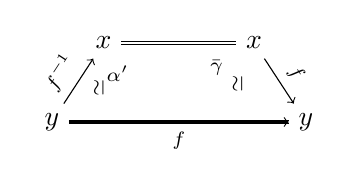
\begin{tikzpicture}[x=1.7em,y=1.3em]
  \node (xl) at (1.1,2.2) {$x$};
  \node (xr) at (4.3,2.2) {$x$};
  \node (yb) at (0,0) {$y$};
  \node (yr) at (5.4,0) {$y$};
  \draw[double] (xl) -- (xr);
  \draw[->] (yb) -- node[above,sloped,pos=0.45]{$\scriptstyle f^{-1}$} (xl);
  \draw[->] (xr) -- node[above,sloped,pos=0.55]{$\scriptstyle f$} (yr);
  \draw[double] (yb) -- (yr);
  \draw[->] (yb) -- node[below]{$\scriptstyle f$} (yr);
  \node at (1.4,1.35) {$\scriptstyle\alpha'$};
  \node[rotate=90] at (1.0,0.95) {$\scriptstyle\simeq$};
  \node at (3.5,1.5) {$\scriptstyle\bar{\gamma}$};
  \node[rotate=90] at (3.95,1.05) {$\scriptstyle\simeq$};
\end{tikzpicture}}
\end{center}
由填充该号角所定义的面正是替代 2-\trSimplex{} $\beta$。这四个 3-\trSimplex{}%
定义了一个映射 $\Lambda^{2}[4]\to A$，其\trFiller{}定义一个 3-\trSimplex{}面，
如下图所示：
\begin{rveq}\label{eq:replacement-3-simplex}
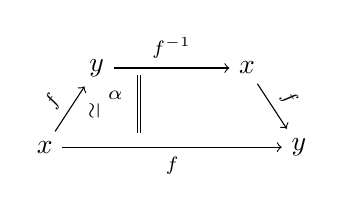
\begin{tikzpicture}[x=1.7em,y=1.3em]
  \node (yt) at (1.1,2.2) {$y$};
  \node (xt) at (4.3,2.2) {$x$};
  \node (xb) at (0,0) {$x$};
  \node (yb) at (5.4,0) {$y$};
  \draw[->] (xb) -- node[above,sloped,pos=0.45]{$\scriptstyle f$} (yt);
  \draw[->] (yt) -- node[above]{$\scriptstyle f^{-1}$} (xt);
  \draw[->] (xt) -- node[above,sloped,pos=0.55]{$\scriptstyle f$} (yb);
  \draw[->] (xb) -- node[below]{$\scriptstyle f$} (yb);
  \node at (1.5,1.45) {$\scriptstyle\alpha$};
  \node[rotate=90] at (1.05,1.0) {$\scriptstyle\simeq$};
  \draw[double] (2.0,2.0) -- (2.0,0.4);
  \node at (2.5,1.1) {$\scriptstyle\lVert$};
\end{tikzpicture}
\qquad\simeq\qquad
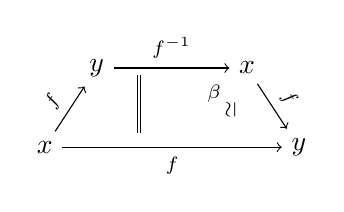
\begin{tikzpicture}[x=1.7em,y=1.3em]
  \node (yt) at (1.1,2.2) {$y$};
  \node (xt) at (4.3,2.2) {$x$};
  \node (xb) at (0,0) {$x$};
  \node (yb) at (5.4,0) {$y$};
  \draw[->] (xb) -- node[above,sloped,pos=0.45]{$\scriptstyle f$} (yt);
  \draw[->] (yt) -- node[above]{$\scriptstyle f^{-1}$} (xt);
  \draw[->] (xt) -- node[above,sloped,pos=0.55]{$\scriptstyle f$} (yb);
  \draw[->] (xb) -- node[below]{$\scriptstyle f$} (yb);
  \node at (3.6,1.5) {$\scriptstyle\beta$};
  \node[rotate=90] at (3.95,1.05) {$\scriptstyle\simeq$};
  \draw[double] (2.0,2.0) -- (2.0,0.4);
  \node at (1.6,1.1) {$\scriptstyle\lVert$};
\end{tikzpicture}
\end{rveq}
这就定义了所需的\trExtension{} $E_{3}^{-}\to A$。
\end{proof}

手持\cref{cor:inner-fillings-complicial-set}，我们现在可以证明 Joyal 的特殊
外\trHorn{}填充结果。

\begin{proof}[\cref{prop:outer-complicial-horn-fillings}的证明]
设 $A$ 是一个自然标记\trQuasiCategory。我们论证：唯一映射 $!\colon A\to\qcOne$
满足\cref{cor:inner-fillings-complicial-set}的假设。对诸内复状号角扩张而言，
全部非退化带标记\trSimplex{}都在维数二或更高，故 $A$ 对它们容有\trFiller——
这仅仅因为\trQuasiCategory{}是对全部内\trHorn{}容有\trFiller{}的%
\trSimplicialSet。由于\trQuasiCategory{}中一对\trIsomorphism{}的复合仍是%
\trIsomorphism，$A$ 沿 $\Delta^{1}[2]'\hookrightarrow_{e}\Delta^{1}[2]''$
容有\trExtension。(D.1.11) 的其余复状薄性扩张是只在维数至少二的\trSimplex{}的
标记上有所不同的\trEntireInclusion；由于全部这样的\trSimplex{}在自然标记下都是薄的，$A$
对它们也容有\trExtension。从而，$A\to\qcOne$ 是一个内复状纤维化。

为作结论，只须论证 $A$ 容有如下形式的\trExtension
\begin{center}
\begin{tikzpicture}[x=1.6em,y=1.4em]
  \node (lt) at (0,1.2) {$\Delta[1]^{\sharp}$};
  \node (rt) at (2.8,1.2) {$A$};
  \node (lb) at (0,-1.2) {$\mathrm{sk}_{2}\qcInt^{\sharp}$};
  \draw[->] (lt) -- node[above]{$\scriptstyle f$} (rt);
  \draw[right hook->] (lb) -- (lt);
  \draw[->,dashed] (0.45,-1.0) -- (2.35,1.0);
\end{tikzpicture}
\end{center}
由于 $A$ 是自然标记的，附贴映射 $f\colon x\to y$ 定义 $A$ 中一个\trIsomorphism。
据第 1 章中的\cref{def:isomorphism-quasi-category}，这意味着存在 2-\trSimplex
\begin{center}
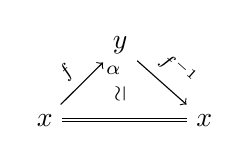
\begin{tikzpicture}[x=1.6em,y=1.35em]
  \node (y) at (1.7,2.0) {$y$};
  \node (xl) at (0,0) {$x$};
  \node (xr) at (3.6,0) {$x$};
  \draw[->] (xl) -- node[above,sloped,pos=0.45]{$\scriptstyle f$} (y);
  \draw[->] (y) -- node[above,sloped,pos=0.55]{$\scriptstyle f^{-1}$} (xr);
  \draw[double] (xl) -- (xr);
  \node at (1.55,1.35) {$\scriptstyle\alpha$};
  \node[rotate=90] at (1.7,0.72) {$\scriptstyle\simeq$};
\end{tikzpicture}
\qquad
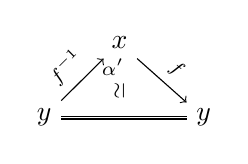
\begin{tikzpicture}[x=1.6em,y=1.35em]
  \node (x) at (1.7,2.0) {$x$};
  \node (yl) at (0,0) {$y$};
  \node (yr) at (3.6,0) {$y$};
  \draw[->] (yl) -- node[above,sloped,pos=0.45]{$\scriptstyle f^{-1}$} (x);
  \draw[->] (x) -- node[above,sloped,pos=0.55]{$\scriptstyle f$} (yr);
  \draw[double] (yl) -- (yr);
  \node at (1.55,1.35) {$\scriptstyle\alpha'$};
  \node[rotate=90] at (1.7,0.72) {$\scriptstyle\simeq$};
\end{tikzpicture}
\end{center}
它们提供了所需\trExtension{} $\mathrm{sk}_{2}\qcInt^{\sharp}\to A$ 的数据。
\end{proof}

这就证明了下述把\trQuasiCategory{}刻画为复状单纯集的定理的困难方向：

\begin{theorem}\label{thm:natural-marking-complicial}
一个\trQuasiCategory{}的自然标记是一个复状单纯集，而且确实是使一个%
\trQuasiCategory{}成为复状单纯集的极大标记。反之，任何「维数高于一的全部%
\trSimplex{}皆被标记」的复状单纯集，其底\trSimplicialSet{}是一个%
\trQuasiCategory。
\end{theorem}

\begin{proof}
\cref{prop:outer-complicial-horn-fillings}表明自然标记\trQuasiCategory{}对诸
外复状号角扩张容有\trFiller，且其证明表明它对诸内复状号角扩张也容有%
\trFiller。如那里所论证，由于自然标记\trQuasiCategory{}是 1-平凡的，维数大于
1 的复状薄性扩张是自动的，而维数 1 的三个复状薄性扩张要求\trQuasiCategory{}%
中的\trIsomorphism{}满足\trTwoOfThreeProperty，后者为真。
从而，自然标记\trQuasiCategory{}是复状单纯集。据\cref{lem:marked-edges-equivalences}，
不可能在 $A$ 中再标记任何额外的边而仍保持复状单纯集的性质，故自然标记就是
极大的那一个。

逆命题是初等的，留给读者，见\cref{ex:underlying-1-trivial-quasi-category}。
\end{proof}

我们现在给出\cref{thm:natural-marking-complicial}的若干示例应用，重访 1.1 节
中的某些结果并利用\cref{prop:outer-complicial-horn-fillings}证明之。例如，我们
回到第 1 章中的\cref{cor:kan-groupoid}：

\begin{corollary}\label{cor:kan-complex-groupoid}
一个\trQuasiCategory{} $A$ 是一个\trKanComplex{}，当且仅当它的%
\trHomotopyCategory{}是一个\trGroupoid。
\end{corollary}

\begin{proof}
显然，\trKanComplex{}的\trHomotopyCategory{}是一个\trGroupoid，故我们把注意力
集中在逆命题上。据\cref{thm:natural-marking-complicial}，一个\trQuasiCategory{}%
可以视为一个复状单纯集，其中维数高于 1 的\trSimplex{}皆被标记，而带标记的边
恰好是诸\trIsomorphism——按定义，\trIsomorphism{}即那些在\trHomotopyCategory{}%
中表示\trIsomorphism{}的 1-\trSimplex。若 $A$ 的\trHomotopyCategory{}是一个%
\trGroupoid，则这告诉我们 $A$ 是极大标记的，而\cref{ex:maximally-marked-kan}观察到：
一个极大标记的
复状单纯集定义一个\trKanComplex。
\end{proof}

对于下一个结果，我们重访第 1 章中的\cref{cor:hc-isomorphism}，并从那里给出的
证明中消除对「由\trQuasiCategory{}中的\trIsomorphism{}张成的极大%
\trKanComplex」的援引——其存在性由特殊外\trHorn{}提升推出。

\begin{corollary}\label{cor:isomorphism-extends-hc-isomorphism}
\trQuasiCategory{} $A$ 中的一支箭头 $f$ 是一个\trIsomorphism，当且仅当它可%
\trExtension{}成一个\trHomotopyCoherentIsomorphism
\begin{center}
\begin{tikzpicture}[x=1.6em,y=1.4em]
  \node (lt) at (0,1.2) {$\qcTwo$};
  \node (rt) at (2.8,1.2) {$A$};
  \node (lb) at (0,-1.2) {$\qcInt$};
  \draw[->] (lt) -- node[above]{$\scriptstyle f$} (rt);
  \draw[right hook->] (lb) -- (lt);
  \draw[->,dashed] (0.45,-1.0) -- (2.35,1.0);
\end{tikzpicture}
\end{center}
\end{corollary}

\begin{proof}
当把\trQuasiCategory{} $A$ 视为自然标记的复状单纯集时，该\trIsomorphism{} $f$
定义一个带标记映射 $f\colon\qcTwo^{\sharp}\to A$。据\cref{lem:marked-anodyne-free-isomorphism}，
单射 $\qcTwo^{\sharp}\hookrightarrow\qcInt^{\sharp}$ 是一支带标记\trAnodyneExtension，从而
$A$ 对该映射可提升。忘掉标记，这就证明了 $A$ 中的每支\trIsomorphism{}都可%
\trExtension{}成一个\trHomotopyCoherentIsomorphism。逆命题由第 1 章中的
\cref{def:isomorphism-quasi-category} 显然可得。
\end{proof}

接下来，我们证明第 1 章中的\cref{cor:exponential-ideal}所陈述的两句话。

\begin{lemma}\label{lem:exponential-naturally-marked}
若 $A$ 是一个自然标记\trQuasiCategory{}且 $X$ 是一个极小标记\trSimplicialSet，
则 $A^{X}$ 是一个自然标记\trQuasiCategory。
\end{lemma}

\begin{proof}
据\cref{prop:marked-cartesian-closed}，$A^{X}$ 中的 $n$-\trSimplex{}对应于映射
$X\times\Delta[n]\to A$。由于定义域是极小标记的，可知 $A^{X}$ 的底%
\trSimplicialSet{}与底\trSimplicialSet{}的指数相重合，从而据
\cref{cor:leibniz-exponential}(i) 定义一个\trQuasiCategory。

为看出 $A^{X}$ 中维数大于一的\trSimplex{}皆被标记，考虑\trExtension{}问题
\begin{center}
\begin{tikzpicture}[x=1.6em,y=1.4em]
  \node (lt) at (0,1.2) {$X\times\Delta[n]$};
  \node (rt) at (3.4,1.2) {$A$};
  \node (lb) at (0,-1.2) {$X\times\Delta[n]_{t}$};
  \draw[->] (lt) -- (rt);
  \draw[right hook->] (lb) -- node[pos=0.5,left]{$\scriptstyle e$} (lt);
  \draw[->,dashed] (0.6,-1.0) -- (2.9,1.0);
\end{tikzpicture}
\end{center}

（$n>1$）。据\cref{prop:marked-cartesian-closed}，在 $X\times\Delta[n]_{t}$ 中
被标记而在 $X\times\Delta[n]$ 中未被标记的\trSimplex{}只有 $n$-\trSimplex，而
由于 $A$ 中全部 $n$-\trSimplex{}都被标记，显然所需的\trExtension{}存在。

据\cref{cor:leibniz-exponential}(ii)，$A^{X}$ 是一个复状单纯集，故据
\cref{lem:marked-edges-equivalences}，$A^{X}$ 中每条带标记的边都是一个%
\trIsomorphism。只剩下表明：\trQuasiCategory{} $A^{X}$ 中的每支\trIsomorphism{}
$f\colon\Delta[1]\to A^{X}$ 都被标记，即容有如下图右下方所示的\trExtension：
\begin{rveq}\label{eq:components-pushout}
\begin{tikzpicture}[x=1.15em,y=1.5em]
  \node (tl) at (0,1.7) {$\coprod\limits_{x\in X_{0}}\Delta[1]$};
  \node (tm) at (6.8,1.7) {$X\times\Delta[1]$};
  \node (tr) at (13.2,1.7) {$A$};
  \node (bl) at (0,-1.5) {$\coprod\limits_{x\in X_{0}}\Delta[1]_{t}$};
  \node (bm) at (6.8,-1.5) {$X\times\Delta[1]_{t}$};
  \draw[->] (tl) -- (tm);
  \draw[->] (tm) to[bend left=18] node[above,pos=0.5]{$\scriptstyle f_{x}$} (tr);
  \draw[right hook->] (tl) -- node[pos=0.5,left]{$\scriptstyle e$} (bl);
  \node at (1.35,0.55) {$\scriptstyle\lrcorner$};
  \draw[->] (bl) -- node[below]{$\scriptstyle(x\sigma^{0},\mathrm{id})$} (bm);
  \draw[right hook->] (tm) -- node[pos=0.5,right]{$\scriptstyle e$} (bm);
  \node at (6.05,-0.15) {$\scriptstyle\llcorner$};
  \draw[->,dashed] (bm) -- node[above,sloped,pos=0.6]{$\scriptstyle f$} (tr);
  \draw[->,dotted] (bm) to[bend right=28] (tr);
\end{tikzpicture}
\end{rveq}
据\cref{prop:marked-cartesian-closed}，在 $X\times\Delta[1]_{t}$ 中被标记而在
$X\times\Delta[1]$ 中未被标记的\trSimplex{}只有这样的 1-\trSimplex：其在 $X$
中的分量是退化的，而其在 $\Delta[1]_{t}$ 中的分量是非退化 1-\trSimplex；上图
左上的那个方块既是\trPullback{}又是\trPushout，正表明了这一点。这样的%
\trSimplex{}在 $A$ 中的像定义了 $f$ 的「分量」，如上图顶行的复合所示。

若 $f$ 是 $A^{X}$ 中的一个\trIsomorphism，则它的每个分量 $f_{x}$——即 $f$ 在
求值函数 $\mathrm{ev}_{x}\colon A^{X}\to A$ 下的像——显然也都是\trIsomorphism，
而这当且仅当每个 $f_{x}$ 在 $A$ 中被标记时成立。这些分量 $f_{x}$ 在 $A$ 中被
标记，当且仅当点线提升存在；而由\trPushout{}的\trUniversalProperty，这等价于
虚线提升的存在，如所需。
\end{proof}

由于\cref{lem:exponential-naturally-marked}，我们可以证明一个常被引用的结果：

\begin{corollary}\label{cor:edge-isomorphism-components}
对任何\trQuasiCategory{} $A$ 与\trSimplicialSet{} $X$，$A^{X}$ 中的一条边是
一个\trIsomorphism，当且仅当它按 $X$ 的诸顶点编号的在 $A$ 中的各个分量都是%
\trIsomorphism。
\end{corollary}

\begin{proof}
把 $A$ 视为自然标记\trQuasiCategory{}且把 $X$ 视为极小标记\trSimplicialSet，
据\cref{lem:exponential-naturally-marked}，$A^{X}$ 中的一个 1-\trSimplex{}被
标记，当且仅当它在\trQuasiCategory{} $A^{X}$ 中定义一个\trIsomorphism。于是
该断言即是：一个 1-\trSimplex{}在 $A^{X}$ 中被标记，当且仅当它的诸分量在 $A$
中被标记。据\cref{prop:marked-cartesian-closed}所给出的指数中标记的定义，一个
1-\trSimplex{} $f\colon\Delta[1]\to A^{X}$ 被标记，当且仅当
\eqref{eq:components-pushout} 的虚线\trExtension{}存在。由该处给出的%
\trPushout，这等价于点线\trExtension{}的存在，而后者恰好说：每个分量 $f_{x}$
在 $A$ 中被标记。
\end{proof}

我们以观察到「带标记\trHomotopyEquivalence{}诱导自然标记拟范畴间的%
\trEquivalence」作结。

\begin{lemma}\label{lem:marked-homotopy-equivalence-induces}
设 $A$ 是一个\trQuasiCategory{}，并设 $I\to J$ 是\trSimplicialSet{}的一个映射，
它可\trExtension{}成极小标记\trSimplicialSet{}之间的一个带标记%
\trHomotopyEquivalence。则诱导映射 $A^{J}\twoheadrightarrow A^{I}$ 是%
\trQuasiCategory{}间的一个\trEquivalence。
\end{lemma}

\begin{proof}
赋予 $A$ 其自然标记，于是据\cref{thm:natural-marking-complicial}它定义一个
复状单纯集。据\cref{ex:restriction-map-equivalence}，$A^{J}\twoheadrightarrow A^{I}$
此时是复状单纯集间的一个\trEquivalence。据\cref{cor:complicial-equivalences-hoc}，
这一\trEquivalence{}的数据可以由映射
\[
A^{J}\to A^{I}\text{，}\quad
A^{I}\to A^{J}\text{，}\quad
A^{I}\to(A^{I})^{\qcInt^{\sharp}}\text{，}\quad
A^{J}\to(A^{J})^{\qcInt^{\sharp}}
\]
给出，而在忘掉标记之后，这份数据便定义了第 1 章中的\cref{def:equivalences-quasi-categories}
的意义下的\trQuasiCategory{}间的一个\trEquivalence。\footnote{注意当 $A$ 是
自然标记\trQuasiCategory{}时 $A^{\qcInt}\cong A^{\qcInt^{\sharp}}$。}
\end{proof}

\begin{digression}[论等价与高维\trSimplex{}的饱和]\label{dig:saturation-higher-simplices}
\cref{lem:marked-edges-equivalences}表明：复状单纯集中的带标记边应当被诠释为
适当意义下的\trEquivalence。类似的诠释对更高维数的带标记\trSimplex{}也是适当
的。于是，我们可以把「一个复状单纯集是 $n$-平凡的」这一条件诠释为要求：维数
$r>n$ 的全部\trSimplex{}都是弱可逆的。

在理解了复状单纯集中的每个带标记\trSimplex{}都是一个\trEquivalence{}之后，
我们便被引向考虑满足其逆条件的复状单纯集，即其中每个\trEquivalence{}都被标记。
这样的\emph{饱和}复状单纯集尤为重要，我们建议用术语 \textbf{$n$-复状单纯集}
（$n$-complicial set）来描述一个 $n$-平凡的饱和复状单纯集（精确定义与若干讨论
见 \cite{bib105} 与 \cite{bib89}）。诸\trKanComplex{}恰好是诸 \emph{0-复状
单纯集}（0-complicial sets），据\cref{ex:maximally-marked-kan}；而%
\trQuasiCategory{}恰好是诸 \emph{1-复状单纯集}（1-complicial sets），据
\cref{thm:natural-marking-complicial}。如这一模式所提示的，诸 \emph{$n$-复状
单纯集}定义了 $(\infty,n)$-范畴的一个表现良好的模型，其意义是：这样的%
\trSimplicialSet{}的全子范畴定义一个\trCartesianClosed{}∞-宇宙，如我们在
\cref{prop:n-complicial-cosmos}中所证明。%
\end{digression}

\subsection*{练习}

\begin{exercise}\label{ex:underlying-1-trivial-quasi-category}
证明：任何 1-平凡复状单纯集的底\trSimplicialSet{}是一个\trQuasiCategory。
\footnote{本结果的一个逆命题式变体见于\cref{thm:natural-marking-complicial}。}
\end{exercise}

\begin{exercise}\label{ex:prove-lem-nerve-1-category}
证明\cref{lem:nerve-1-category-complicial}。
\end{exercise}

\begin{exercise}\label{ex:two-of-six-simplex}
设 $\Delta[3]_{\mathrm{eq}}$ 表示「三取六 3-\trSimplex」（2-of-6 3-simplex），
其中边 $\{02\}$ 与 $\{13\}$ 以及维数大于 1 的全部\trSimplex{}都被标记。证明：
\begin{enumerate}[label=(\roman*)]
\item 复状单纯集 $A$ 中的一个 1-\trSimplex{}是一个\trEquivalence，当且仅当它
  定义 3-\trSimplex{} $\Delta[3]_{\mathrm{eq}}\to A$ 的 $\{12\}$-边。
\item 一个复状单纯集是 1-饱和的，当且仅当它沿\trEntireInclusion
\begin{center}
\begin{tikzpicture}[x=1.6em,y=1.4em]
  \node (lt) at (0,1.2) {$\Delta[3]_{\mathrm{eq}}$};
  \node (rt) at (3.0,1.2) {$A$};
  \node (lb) at (0,-1.2) {$\Delta[3]^{\sharp}$};
  \draw[->] (lt) -- (rt);
  \draw[right hook->] (lb) -- node[pos=0.5,left]{$\scriptstyle e$} (lt);
  \draw[->,dashed] (0.6,-1.0) -- (2.5,1.0);
\end{tikzpicture}
\end{center}
  容有\trExtension。
\end{enumerate}
\end{exercise}












